% Options for packages loaded elsewhere
\PassOptionsToPackage{unicode}{hyperref}
\PassOptionsToPackage{hyphens}{url}
%
\documentclass[
]{book}
\usepackage{amsmath,amssymb}
\usepackage{iftex}
\ifPDFTeX
  \usepackage[T1]{fontenc}
  \usepackage[utf8]{inputenc}
  \usepackage{textcomp} % provide euro and other symbols
\else % if luatex or xetex
  \usepackage{unicode-math} % this also loads fontspec
  \defaultfontfeatures{Scale=MatchLowercase}
  \defaultfontfeatures[\rmfamily]{Ligatures=TeX,Scale=1}
\fi
\usepackage{lmodern}
\ifPDFTeX\else
  % xetex/luatex font selection
\fi
% Use upquote if available, for straight quotes in verbatim environments
\IfFileExists{upquote.sty}{\usepackage{upquote}}{}
\IfFileExists{microtype.sty}{% use microtype if available
  \usepackage[]{microtype}
  \UseMicrotypeSet[protrusion]{basicmath} % disable protrusion for tt fonts
}{}
\makeatletter
\@ifundefined{KOMAClassName}{% if non-KOMA class
  \IfFileExists{parskip.sty}{%
    \usepackage{parskip}
  }{% else
    \setlength{\parindent}{0pt}
    \setlength{\parskip}{6pt plus 2pt minus 1pt}}
}{% if KOMA class
  \KOMAoptions{parskip=half}}
\makeatother
\usepackage{xcolor}
\usepackage{longtable,booktabs,array}
\usepackage{calc} % for calculating minipage widths
% Correct order of tables after \paragraph or \subparagraph
\usepackage{etoolbox}
\makeatletter
\patchcmd\longtable{\par}{\if@noskipsec\mbox{}\fi\par}{}{}
\makeatother
% Allow footnotes in longtable head/foot
\IfFileExists{footnotehyper.sty}{\usepackage{footnotehyper}}{\usepackage{footnote}}
\makesavenoteenv{longtable}
\usepackage{graphicx}
\makeatletter
\def\maxwidth{\ifdim\Gin@nat@width>\linewidth\linewidth\else\Gin@nat@width\fi}
\def\maxheight{\ifdim\Gin@nat@height>\textheight\textheight\else\Gin@nat@height\fi}
\makeatother
% Scale images if necessary, so that they will not overflow the page
% margins by default, and it is still possible to overwrite the defaults
% using explicit options in \includegraphics[width, height, ...]{}
\setkeys{Gin}{width=\maxwidth,height=\maxheight,keepaspectratio}
% Set default figure placement to htbp
\makeatletter
\def\fps@figure{htbp}
\makeatother
\setlength{\emergencystretch}{3em} % prevent overfull lines
\providecommand{\tightlist}{%
  \setlength{\itemsep}{0pt}\setlength{\parskip}{0pt}}
\setcounter{secnumdepth}{5}
\usepackage{booktabs}
\usepackage{amsthm}
\makeatletter
\def\thm@space@setup{%
  \thm@preskip=8pt plus 2pt minus 4pt
  \thm@postskip=\thm@preskip
}
\makeatother
\ifLuaTeX
  \usepackage{selnolig}  % disable illegal ligatures
\fi
\usepackage[]{natbib}
\bibliographystyle{apalike}
\IfFileExists{bookmark.sty}{\usepackage{bookmark}}{\usepackage{hyperref}}
\IfFileExists{xurl.sty}{\usepackage{xurl}}{} % add URL line breaks if available
\urlstyle{same}
\hypersetup{
  pdftitle={Optimal Control and Estimation},
  pdfauthor={Heng Yang},
  hidelinks,
  pdfcreator={LaTeX via pandoc}}

\title{Optimal Control and Estimation}
\author{Heng Yang}
\date{2023-06-13}

\usepackage{amsthm}
\newtheorem{theorem}{Theorem}[chapter]
\newtheorem{lemma}{Lemma}[chapter]
\newtheorem{corollary}{Corollary}[chapter]
\newtheorem{proposition}{Proposition}[chapter]
\newtheorem{conjecture}{Conjecture}[chapter]
\theoremstyle{definition}
\newtheorem{definition}{Definition}[chapter]
\theoremstyle{definition}
\newtheorem{example}{Example}[chapter]
\theoremstyle{definition}
\newtheorem{exercise}{Exercise}[chapter]
\theoremstyle{definition}
\newtheorem{hypothesis}{Hypothesis}[chapter]
\theoremstyle{remark}
\newtheorem*{remark}{Remark}
\newtheorem*{solution}{Solution}
\begin{document}
\maketitle

{
\setcounter{tocdepth}{1}
\tableofcontents
}
\hypertarget{preface}{%
\chapter*{Preface}\label{preface}}
\addcontentsline{toc}{chapter}{Preface}

This is the textbook for Harvard ES/AM 158: Introduction to Optimal Control and Estimation. Information about the offerings of the class is listed below.

\hypertarget{fall}{%
\subsubsection*{2023 Fall}\label{fall}}
\addcontentsline{toc}{subsubsection}{2023 Fall}

\textbf{Time}: Mon/Wed 2:15 - 3:30pm

\textbf{Location}: Science and Engineering Complex, Room TBD

\textbf{Instructor}: \href{https://hankyang.seas.harvard.edu/}{Heng Yang}

\textbf{Teaching Fellow}: \href{https://scholar.harvard.edu/weiyuli/home}{Weiyu Li}

\href{https://docs.google.com/document/d/1q8_jB5dLx9jHOBi3DQ48Vv2E243ocGCGm_H0mJuOojM/edit?usp=sharing}{\textbf{Syllabus}}

\hypertarget{acknowledgment}{%
\subsubsection*{Acknowledgment}\label{acknowledgment}}
\addcontentsline{toc}{subsubsection}{Acknowledgment}

\hypertarget{formulation}{%
\chapter{The Optimal Control Formulation}\label{formulation}}

\hypertarget{the-basic-problem}{%
\section{The Basic Problem}\label{the-basic-problem}}

Consider a discrete-time dynamical system
\begin{equation}
x_{k+1} = f_k (x_k, u_k, w_k), \quad k =0,1,\dots,N-1
\label{eq:discrete-time-dynamics}
\end{equation}
where

\begin{itemize}
\item
  \(x_k \in \mathbb{X} \subseteq \mathbb{R}^n\) is the \emph{state} of the system,
\item
  \(u_k \in \mathbb{U} \subseteq \mathbb{R}^m\) is the \emph{control} we wish to design,
\item
  \(w_k \in \mathbb{W} \subseteq \mathbb{R}^p\) a random \emph{disturbance} or noise (e.g., due to unmodelled dynamics) which is described by a probability distribution \(P_k(\cdot \mid x_k, u_k)\) that may depend on \(x_k\) and \(u_k\) but not on prior disturbances \(w_0,\dots,w_{k-1}\),
\item
  \(k\) indexes the discrete time,
\item
  \(N\) denotes the horizon,
\item
  \(f_k\) models the transition function of the system (typically \(f_k \equiv f\) is time-invariant, especially for robotics systems; we use \(f_k\) here to keep full generality).
\end{itemize}

\begin{remark}[Deterministic v.s. Stochastic]
When \(w_k \equiv 0\) for all \(k\), we say the system \eqref{eq:discrete-time-dynamics} is \emph{deterministic}; otherwise we say the system is \emph{stochastic}. In the following we will deal with the stochastic case, but most of the methodology should carry over to the deterministic setup.
\end{remark}

We consider the class of \emph{controllers} (also called \emph{policies}) that consist of a sequence of functions
\[
\pi = \{ \mu_0,\dots,\mu_{N-1} \},
\]
where \(\mu_k (x_k) \in \mathbb{U}\) for all \(x_k\), i.e., \(\mu_k\) is a \emph{feedback} controller that maps the state to an admissible control. Given an initial state \(x_0\) and an admissible policy \(\pi\), the state \emph{trajectory} of the system is a sequence of random variables that evolve according to
\begin{equation}
x_{k+1} = f_k(x_k,\mu_k(x_k),w_k), \quad k=0,\dots,N-1
\label{eq:closed-loop-state-trajectory}
\end{equation}
where the randomness comes from the disturbance \(w_k\).

We assume the state-control trajectory \(\{u_k\}_{k=0}^{N-1}\) and \(\{x_k \}_{k=0}^{N}\) induce an \emph{additive cost}
\begin{equation}
g_N(x_N) + \sum_{k=0}^{N-1} g_k(x_k,u_k)
\label{eq:additive-cost}
\end{equation}
where \(g_k,k=0,\dots,N\) are some user-designed functions.

With \eqref{eq:closed-loop-state-trajectory} and \eqref{eq:additive-cost}, for any admissible policy \(\pi\), we denote its induced \emph{expected cost} with initial state \(x_0\) as
\begin{equation}
J_\pi (x_0) = \mathbb{E} \left\{ g_N(x_N) + \sum_{k=0}^{N-1} g_k (x_k, \mu_k(x_k))  \right\},
\label{eq:expected-cost}
\end{equation}
where the expectation is taken over the randomness of \(w_k\).

\begin{definition}[Discrete-time, Finite-horizon Optimal Control]
\protect\hypertarget{def:basicproblem}{}\label{def:basicproblem}Find the best admissible controller that minimizes the expected cost in \eqref{eq:expected-cost}
\begin{equation}
\pi^\star \in \arg\min_{\pi \in \Pi} J_\pi(x_0),
\end{equation}
where \(\Pi\) is the set of all admissible controllers.
The cost attained by the optimal controller, i.e., \(J^\star = J_{\pi^\star}(x_0)\) is called the optimal \emph{cost-to-go}, or the optimal \emph{value function}.
\end{definition}

\hypertarget{open-loop-v.s.-closed-loop}{%
\section{Open-Loop v.s. Closed-Loop}\label{open-loop-v.s.-closed-loop}}

An important feature of the basic problem in Definition \ref{def:basicproblem}

\hypertarget{stability}{%
\chapter{Stability Analysis}\label{stability}}

\begin{lemma}[Barbalat's Lemma]
\protect\hypertarget{lem:Barbalat}{}\label{lem:Barbalat}Let \(f(t)\) be differentiable, if

\begin{itemize}
\item
  \(\lim_{t \rightarrow \infty} f(t)\) is finite, and
\item
  \(\dot{f}(t)\) is uniformly continuous,\footnote{A sufficient condition for this to hold is that \(\ddot{f}\) exists and is bounded.}
\end{itemize}

then
\[
\lim_{t \rightarrow \infty} \dot{f}(t) = 0.
\]
\end{lemma}

\begin{theorem}[Barbalat's Stability Certificate]
\protect\hypertarget{thm:BarbalatStability}{}\label{thm:BarbalatStability}If a scalar function \(V(x,t)\) satisfies

\begin{itemize}
\item
  \(V(x,t)\) is lower bounded,
\item
  \(\dot{V}(x,t)\) is negative semidefinite
\item
  \(\dot{V}(x,t)\) is uniformly continuous
\end{itemize}

then \(\dot{V}(x,t) \rightarrow 0\) as \(t \rightarrow \infty\).
\end{theorem}

\begin{proof}
\(V(x,t)\) is lower bounded and \(\dot{V}\) is negative semidefinite implies the limit of \(V\) as \(t \rightarrow \infty\) is finite (note that \(V(x,t) \leq V(x(0),0)\)). Then the theorem clearly follows from Barbalat's Lemma \ref{lem:Barbalat}.
\end{proof}

\hypertarget{adaptivecontrol}{%
\chapter{Adaptive Control}\label{adaptivecontrol}}

\hypertarget{model-reference-adaptive-control}{%
\section{Model-Reference Adaptive Control}\label{model-reference-adaptive-control}}

Basic flow for designing an adaptive controller

\begin{enumerate}
\def\labelenumi{\arabic{enumi}.}
\item
  Design a control law with variable parameters
\item
  Design an adaptation law for adjusting the control parameters
\item
  Analyze the convergence of the closed-loop system
\end{enumerate}

The control law design at the first step typically requires the designer to know what a good controller is if the true parameters were actually known, e.g., from feedback linearization (Appendix \ref{feedbacklinearization}), sliding control (Appendix \ref{slidingcontrol}) etc.

The design of the adaptation law typically comes from analyzing the dynamics of the tracking error, which as we will see often appears in the form of Lemma \ref{lem:adaptivecontrolbasic}.

The convergence of the closed-loop system is usually analyzed with the help of a Lyapunov-like function introduced in Chapter \ref{stability}.

\begin{lemma}[Basic Lemma]
\protect\hypertarget{lem:adaptivecontrolbasic}{}\label{lem:adaptivecontrolbasic}Let two signals \(e(t)\) and \(\phi(t)\) be related by
\begin{equation}
e(t) = H(p)[k \phi(t)^T v(t)]
\label{eq:acbasiclemmaephi}
\end{equation}
where \(e(t)\) a scalar output signal, \(H(p)\) a strictly positive real (SPR) transfer function, \(k\) an unknown real number with known sign, \(\phi(t) \in \mathbb{R}^m\) a control signal, and \(v(t) \in \mathbb{R}^m\) a measurable input signal.

If the control signal \(\phi(t)\) satisfies
\begin{equation}
\dot{\phi}(t) = - \mathrm{sgn}(k) \gamma e(t) v(t)
\label{eq:acbasiclemmaphilaw}
\end{equation}
with \(\gamma > 0\) a positive constant, then \(e(t)\) and \(\phi(t)\) are globally bounded. Moreover, if \(v(t)\) is bounded, then
\[
\lim_{t \rightarrow \infty} e(t) = 0.
\]
\end{lemma}

\begin{proof}
Let the state-space representation of \eqref{eq:acbasiclemmaephi} be
\begin{equation}
\dot{x} = A x + b [k \phi^T v], \quad e = c^T x.
\label{eq:acbasiclemmastatespace}
\end{equation}
Since \(H(p)\) is SPR, it follows from the Kalman-Yakubovich Lemma \ref{lem:KalmanYakubovich} that there exist \(P,Q \succ 0\) such that
\[
A^T P + P A = -Q, \quad Pb = c.
\]
Let
\[
V(x,\phi) = x^T P x + \frac{|k|}{\gamma} \phi^T \phi,
\]
clearly \(V\) is positive definite (i.e., \(V(0,0)=0\), and \(V(x,\phi) > 0\) for all \(x \neq 0, \phi \neq 0\)). The time derivative of \(V\) along the trajectory defined by \eqref{eq:acbasiclemmastatespace} with \(\phi\) chosen as in \eqref{eq:acbasiclemmaphilaw} is
\begin{align}
\dot{V} & = \frac{\partial V}{\partial x} \dot{x} + \frac{\partial V}{\partial \phi} \dot{\phi} \\
&= x^T (PA + A^T P) x + 2 x^T P b (k \phi^T v) + \frac{2|k|}{\gamma} \phi^T (- \mathrm{sgn}(k) \gamma e v) \\
& = - x^T Q x + 2 (x^T c)(k\phi^T v) - 2 \phi^T (e v) \\
& = - x^T Q x \leq 0.
\end{align}
As a result, we know \(x\) and \(\phi\) must be bounded (\(V(x(t),\phi(t)) \leq V(x(0),\phi(0))\) is bounded). Since \(e = c^T x\), we know \(e\) must be bounded as well.

If the input signal \(v\) is also bounded, then \(\dot{x}\) is bounded as seen from \eqref{eq:acbasiclemmastatespace}. Because \(\ddot{V} = -2x^T Q \dot{x}\) is now bounded, we know \(\dot{V}\) is uniformly continuous. Therefore, by Barbalat's stability certificate (Theorem \ref{thm:BarbalatStability}), we know \(\dot{V}\) tends to zero as \(t\) tends to infinity, which implies \(\lim_{t \rightarrow \infty} x(t) = 0\) and hence \(\lim_{t \rightarrow \infty} e(t) = 0\).
\end{proof}

\hypertarget{first-order-systems}{%
\subsection{First-Order Systems}\label{first-order-systems}}

Consider the first-order single-input single-output (SISO) system
\begin{equation}
\dot{x} = - a x + b u
\label{eq:ac-first-linear}
\end{equation}
where \(a\) and \(b\) are unknown groundtruth parameters. However, we do assume that the sign of \(b\) is known. {What if the sign of \(b\) is unknown too?}

Let \(r(t)\) be a reference trajectory, e.g., a step function or a sinusoidal function, and \(x_d(t)\) be a desired system trajectory that tracks the reference
\begin{equation}
\dot{x}_d = - a_d x_d + b_d r(t),
\label{eq:ac-first-linear-desired}
\end{equation}
where \(a_d,b_d > 0\) are user-defined constants. Note that the transfer function from \(r\) to \(x_d\) is
\[
x_d = \frac{b_d}{p + a_d} r
\]
and the system is stable. {Review basics of transfer function.}

The goal of adaptive control is to design a control law and an adaptation law such that the tracking error of the system \(x(t) - x_d(t)\) converges to zero.

\textbf{Control law}. We design the control law as
\begin{equation}
u = \hat{a}_r(t) r + \hat{a}_x(t) x 
\label{eq:ac-first-linear-control}
\end{equation}
where \(\hat{a}_r(t)\) and \(\hat{a}_x(t)\) are time-varying feedback gains that we wish to adapt. The closed-loop dynamics of system \eqref{eq:ac-first-linear} with the controller \eqref{eq:ac-first-linear-control} is
\[
\dot{x} = - a x + b (\hat{a}_r r + \hat{a}_x x) = - (a - b \hat{a}_x) x + b \hat{a}_r r. 
\]
With the equation above,
the reason for choosing the control law \eqref{eq:ac-first-linear-control} is clear: if the system parameters \((a,b)\) were known, then choosing
\begin{equation}
a_r^\star = \frac{b_d}{b}, \quad a_x^\star = \frac{a - a_d}{b}
\label{eq:ac-first-linear-optimal-gain}
\end{equation}
leads to the closed-loop dynamics \(\dot{x} = - a_d x + b_d r\) that is exactly what we want in \eqref{eq:ac-first-linear-desired}.

However, in adaptive control, since the true parameters \((a,b)\) are not revealed to the control designer, an adaptation law is needed to dynamically adjust the gains \(\hat{a}_r\) and \(\hat{a}_x\) based on the tracking error \(x(t) - x_d(t)\).

\textbf{Adaptation law}. Let \(e(t) = x(t) - x_d(t)\) be the tracking error, and we develop its time derivative
\begin{align}
\dot{e} &= \dot{x} - \dot{x}_d \\
        &= - a_d (x - x_d) + (a_d - a + b\hat{a}_x)x + (b \hat{a}_r - b_d) r \\
        & = - a_d e + b\underbrace{(\hat{a}_x - \hat{a}_x^\star)}_{=:\tilde{a}_x} x + b \underbrace{(\hat{a}_r - \hat{a}_r^\star )}_{=:\tilde{a}_r} r \\
        & = - a_d e + b (\tilde{a}_x x + \tilde{a}_r r) \label{eq:ac-first-linear-error-dynamics}
\end{align}
where \(\tilde{a}_x\) and \(\tilde{a}_r\) are the gain errors w.r.t. the optimal gains in \eqref{eq:ac-first-linear-optimal-gain} if the true parameters were known. The error dynamics \eqref{eq:ac-first-linear-error-dynamics} is equivalent to the following transfer function
\begin{equation}
e = \frac{1}{p + a_d} b(\tilde{a}_x x + \tilde{a}_r r) = \frac{1}{p + a_d} \left(b 
\begin{bmatrix} \tilde{a}_x \\ \tilde{a}_r \end{bmatrix}^T 
\begin{bmatrix} x \\ r \end{bmatrix}
\right),
\label{eq:ac-first-linear-error-dynamics-transfer}
\end{equation}
which is in the form of \eqref{eq:acbasiclemmaephi}. Therefore, we choose the adaptation law
\begin{equation}
\begin{bmatrix} \dot{\tilde{a}}_x \\ \dot{\tilde{a}}_r \end{bmatrix} = - \mathrm{sgn}(b) \gamma e \begin{bmatrix} x \\ r \end{bmatrix}.
\label{eq:ac-first-linear-adaptation-law}
\end{equation}

\textbf{Tracking convergence}. With the control law \eqref{eq:ac-first-linear-control} and the adaptation law \eqref{eq:ac-first-linear-adaptation-law}, we can prove that the tracking error converges to zero, using Lemma \ref{lem:adaptivecontrolbasic}. With \(\tilde{a}=[\tilde{a}_x, \tilde{a}_r]^T\), let
\begin{equation}
V(e,\tilde{a}) = e^2 + \frac{|b|}{\gamma} \tilde{a}^T \tilde{a}
\label{eq:ac-first-linear-lyapunov}
\end{equation}
be a positive definite Lyapunov function candidate with time derivative
\[
\dot{V} = - 2a_d e^2 \leq 0.
\]
Clearly, \(e\) and \(\tilde{a}\) are both bounded. Assuming the reference trajectory \(r\) is bounded, we know \(x_d\) is bounded (due to \eqref{eq:ac-first-linear-desired}) and hence \(x\) is bounded (due to \(e = x - x_d\) being bounded). Consequently, from the error dynamics \eqref{eq:ac-first-linear-error-dynamics} we know \(\dot{e}\) is bounded, which implies \(\ddot{V} = -4a_d e \dot{e}\) is bounded and \(\dot{V}\) is uniformly continuous. By Barbalat's stability certificate \ref{thm:BarbalatStability}, we conlude \(e(t) \rightarrow 0\) as \(t \rightarrow \infty\).

It is always better to combine mathematical analysis with intuitive understanding. Can you explain intuitively why the adaptation law \eqref{eq:ac-first-linear-adaptation-law} makes sense? (Hint: think about how the control should react to a negative/positive tracking error.)

\textbf{Parameter convergence}. We have shown the control law \eqref{eq:ac-first-linear-control} and the adaptation law \eqref{eq:ac-first-linear-adaptation-law} guarantee to track the reference trajectory. However, is it guaranteed that the gains of the controller \eqref{eq:ac-first-linear-control} also converge to the optimal gains in \eqref{eq:ac-first-linear-optimal-gain}?

We will now show that the answer is indefinite and it depends on the reference trajectory \(r(t)\). Because the tracking error \(e\) converges to zero, and \(e\) is the output of a stable filter \eqref{eq:ac-first-linear-error-dynamics-transfer}, we know the input \(b(\tilde{a}_x x + \tilde{a}_r r)\) must also converge to zero. On the other hand, the adaptation law \eqref{eq:ac-first-linear-adaptation-law} shows that both \(\dot{\tilde{a}}_x\) and \(\dot{\tilde{a}}_r\) converge to zero (due to \(e\) converging to zero and \(x\), \(r\) being bounded). As a result, we know \(\tilde{a} = [\tilde{a}_x,\tilde{a}_r]^T\) converges to a constant that satisfies
\begin{equation}
v^T \tilde{a} = 0, \quad v = \begin{bmatrix} x \\ r \end{bmatrix},
\label{eq:ac-first-linear-parameter-equation}
\end{equation}
which is a single linear equation of \(\tilde{a}\) with time-varying coeffients.

\begin{itemize}
\item
  \textbf{Constant reference: no guaranteed convergence}. Suppose \(r(t) \equiv r_0 \neq 0\) for all \(t\). From \eqref{eq:ac-first-linear-desired} we know \(x = x_d = \alpha r_0\) when \(t \rightarrow \infty\), where \(\alpha\) is the constant DC gain of the stable filter. Therefore, the linear equation \eqref{eq:ac-first-linear-parameter-equation} reduces to
  \[
  \alpha \tilde{a}_x + \tilde{a}_r  = 0. 
  \]
  This implies that \(\tilde{a}\) does not necessarily converge to zero. In fact, it converges to a straight line in the parameter space.
\item
  \textbf{Persistent excitation: guaranteed convergence}. However, when the signal \(v\) satisfies the so-called \emph{persistent excitation} condition, which states that for any \(t\), there exists \(T, \beta > 0\) such that
  \begin{equation}
  \int_{t}^{t+T} v v^T d\tau \geq \beta I,
  \label{eq:ac-first-linear-persistent-excitation}
  \end{equation}
  then \(\tilde{a}\) is guaranteed to converge to zero. To see this, we multiply \eqref{eq:ac-first-linear-parameter-equation} by \(v\) and integrate it from \(t\) to \(t+T\), which gives rise to
  \[
  \left( \int_{t}^{t+T} vv^T d\tau \right) \tilde{a} = 0.
  \]
  By the persistent excitation condition \eqref{eq:ac-first-linear-persistent-excitation}, we infer that \(\tilde{a} = 0\) is the only solution.
\end{itemize}

It remains to understand under what conditions of the reference trajectory \(r(t)\) can we guarantee the persistent excitation of \(v\). We leave it as an exercise for the reader to show, if \(r(t)\) contains at least one sinusoidal component, then the persistent excitation condition of \(v\) is guaranteed.

\begin{exercise}[Extension to Nonlinear Systems]
\protect\hypertarget{exr:adaptivecontrolfirstordernonlinearsystem}{}\label{exr:adaptivecontrolfirstordernonlinearsystem}Design a control law and an adaptation law for the following system
\[
\dot{x} = - a x - c f(x) + b u
\]
with unknown true parameters \((a,b,c)\) (assume the sign of \(b\) is known) and known nonlinearity \(f(x)\) to track a reference trajectory \(r(t)\). Analyze the convergence of tracking error and parameter estimation error.
\end{exercise}

\hypertarget{high-order-systems}{%
\subsection{High-Order Systems}\label{high-order-systems}}

Consider an \(n\)-th order nonlinear system
\begin{equation}
q^{(n)} + \sum_{i=1}^n \alpha_i f_i(x,t) = bu
\label{eq:ac-singleinput-nonlinear}
\end{equation}
where \(x=[q,\dot{q},\ddot{q},\dots,q^{(n-1)}]^T\) is the state of the system, \(f_i\)'s are known nonlinearities, \((\alpha_1,\dots,\alpha_n,b)\) are unknown parameters of the system (with \(\mathrm{sgn}(b)\) known).

The goal of adaptive control is to control the system \eqref{eq:ac-singleinput-nonlinear} trajectory to follow a desired trajectory \(q_d(t)\) despite no knowing the true parameters.

To facilitate the derivation of the adaptive controller, let us divide both sides of \eqref{eq:ac-singleinput-nonlinear} by \(b\)
\begin{equation}
h q^{(n)} + \sum_{i=1}^n a_i f_i(x,t) = u
\label{eq:ac-singleinput-nonlinear-equivalent}
\end{equation}
where \(h = 1 / b\) and \(a_i = \alpha_i / b\).

\textbf{Control law}. Recall that the choice of the control law is tyically inspired by the control design if the true system parameters were known. We will borrow ideas from sliding control (Appendix \ref{slidingcontrol}).

\begin{itemize}
\item
  \textbf{Known parameters}. Let \(e = q(t) - q_d(t)\) be the tracking error, and define the following combined error
  \[
  s = e^{(n-1)} + \lambda_{n-2} e^{(n-2)} + \dots + \lambda_0 e = \Delta(p) e 
  \]
  where \(\Delta(p) = p^{n-1} + \lambda_{n-2} p^{(n-2)} + \dots + \lambda_0\) is a stable polynomial with user-chosen coeffients \(\lambda_0,\dots,\lambda_{n-2}\). The rationale for defining the combined error \(s\) is that the convergence of \(e\) to zero can be guaranteed by the convergence of \(s\) to zero (when \(\Delta(p)\) is stable).
  Note that \(s\) can be equivalently written as
  \begin{align}
  s & = (q^{(n-1)} - q_d^{(n-1)}) + \lambda_{n-2} e^{(n-2)} + \dots + \lambda_0 e \\
  & = q^{(n-1)} - \underbrace{ \left( q_d^{(n-1)} - \lambda_{n-2} e^{(n-2)} - \dots - \lambda_0 e  \right) }_{q_r^{(n-1)}}.
  \end{align}
  Now consider the control law
  \begin{equation}
  u = h q_r^{(n)} - ks + \sum_{i=1}^n a_i f_i(x,t)
  \label{eq:ac-singleinput-nonlinear-control-law-knownparam}
  \end{equation}
  where
  \[
  q_r^{(n)} = q_d^{(n)} - \lambda_{n-2} e^{(n-1)} - \dots - \lambda_0 \dot{e}
  \]
  and \(k\) is a design constant that has the same sign as \(h\). This choice of control, plugged into the system dynamics \eqref{eq:ac-singleinput-nonlinear-equivalent}, leads to
  \begin{align}
  h q^{(n)} + \sum_{i=1}^n a_i f_i(x,t) = h q_r^{(n)} - ks + \sum_{i=1}^n a_i f_i(x,t) \Longleftrightarrow \\
  h \left( q^{(n)} - q_r^{(n)} \right) + ks = 0 \Longleftrightarrow \\
  h \dot{s} + ks = 0,
  \end{align}
  which guarantees the exponential convergence of \(s\) to zero (note that \(h\) and \(k\) have the same sign), and hence the convergence of \(e\) to zero.
\item
  \textbf{Unknown parameters}. Inspired by the control law with known parameters in \eqref{eq:ac-singleinput-nonlinear-control-law-knownparam}, we design the adapative control law as
  \begin{equation}
  u = \hat{h} q_r^{(n)} - ks + \sum_{i=1}^n \hat{a}_i f_i(x,t),
  \label{eq:ac-singleinput-nonlinear-control-law-unknownparam}
  \end{equation}
  where the time-varying gains \(\hat{h},\hat{a}_1,\dots,\hat{a}_n\) will be adjusted by an adaptation law.
\end{itemize}

\textbf{Adaptation law}. Inserting the adapative control law \eqref{eq:ac-singleinput-nonlinear-control-law-unknownparam} into the system dynamics \eqref{eq:ac-singleinput-nonlinear-equivalent}, we obtain
\begin{align}
h \dot{s} + ks = \tilde{h} q_r^{(n)} + \sum_{i=1}^n \tilde{a}_i f_i (x,t) \Longleftrightarrow \\
s = \frac{1}{p + k/h} \frac{1}{h} \underbrace{ \left( 
    \begin{bmatrix} \tilde{h} \\ \tilde{a}_1 \\ \vdots \\ \tilde{a}_n \end{bmatrix}^T
    \begin{bmatrix} q_r^{(n)} \\ f_1(x,t) \\ \vdots \\ f_n(x,t) \end{bmatrix}
    \right)}_{=:\phi^T v}
\label{eq:ac-singleinput-nonlinear-error-dynamics}
\end{align}
where \(\tilde{h} = \hat{h} - h\) and \(\tilde{a}_i = \hat{a}_i - a_i,i=1,\dots,n\). Again, \eqref{eq:ac-singleinput-nonlinear-error-dynamics} is in the familiar form of \eqref{eq:acbasiclemmaephi}, which naturally leads to the following adaptation law with \(\gamma > 0\) a chosen constant
\begin{equation}
\dot{\phi} = \begin{bmatrix} \dot{\tilde{h}} \\ \dot{\tilde{a}}_1 \\ \vdots \\ \dot{\tilde{a}}_n \end{bmatrix} = - \mathrm{sgn}(h) \gamma s \begin{bmatrix} q_r^{(n)} \\ f_1(x,t) \\ \vdots \\ f_n(x,t) \end{bmatrix}.
\label{eq:ac-singleinput-nonlinear-adaptation-law}
\end{equation}

\textbf{Tracking and parameter convergence}. With the following Lyapunov function
\begin{equation}
V(s,\phi) = |h| s^2 + \frac{1}{\gamma} \phi^T \phi, \quad \dot{V}(s,\phi) -2|k| s^2,
\label{eq:ac-singleinput-nonlinear-lyapunov}
\end{equation}
the global convergence of \(s\) to zero can be easily shown. For parameter convergence, it is easy to see that when \(v\) satisfies the persistent excitation condition, we have that \(\phi\) converges to zero. (However, the relationship between the reference trajectory \(q_d(t)\) and the persistent excitation of \(v\) becomes nontrivial due to the nonlinearities \(f_i\).)

\hypertarget{robotic-manipulator}{%
\subsection{Robotic Manipulator}\label{robotic-manipulator}}

So far our focus has been on systems with a single input (\(u \in \mathbb{R}\)). In the following, we will show that similar techniques can be applied to adapative control of systems with multiple inputs, particularly, trajectory control of a robotic manipulator.

Let \(q \in \mathbb{R}^n\) be the joint angles of a multi-link robotic arm, and \(\dot{q} \in \mathbb{R}^n\) be the joint velocities. The dynamics of a robotic manipulator reads
\begin{equation}
H(q) \ddot{q} + C(q,\dot{q})\dot{q} + g(q) = \tau,
\label{eq:ac-mrac-manipulator-dynamics}
\end{equation}
where \(H(q) \in \mathbb{S}^{n}_{++}\) is the manipulator inertia matrix (that is positive definite), \(C(q,\dot{q})\dot{q}\) is a vector of centripetal and Coriolis torques (with \(C(q,\dot{q}) \in \mathbb{R}^{n \times n}\)), and \(g(q)\) denotes gravitational torques.

\begin{figure}

{\centering 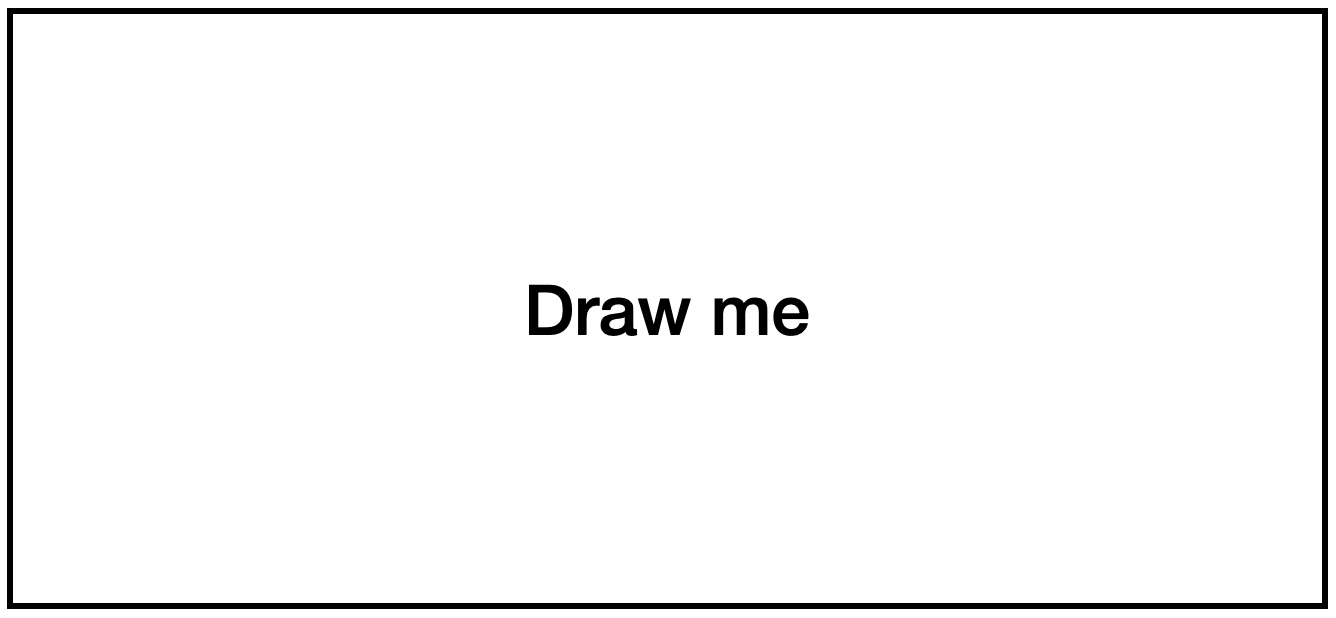
\includegraphics[width=0.6\linewidth]{images/drawme} 

}

\caption{Planar two-link manipulator}\label{fig:planar-two-link}
\end{figure}

\begin{example}[Planar Two-link Manipulator]
\protect\hypertarget{exm:planartwolinkmanipulator}{}\label{exm:planartwolinkmanipulator}The dynamics of a planar two-link manipulator in Fig. \ref{fig:planar-two-link} is
\begin{equation}
\begin{bmatrix} H_{11} & H_{12} \\ H_{21} & H_{22} \end{bmatrix}
\begin{bmatrix} \ddot{q}_1 \\ \ddot{q}_2 \end{bmatrix}
+ 
\begin{bmatrix} - h \dot{q}_2 & -h (\dot{q}_1 + \dot{q}_2) \\ h \dot{q}_1 & 0 \end{bmatrix}
\begin{bmatrix} \dot{q}_1 \\ \dot{q}_2 \end{bmatrix}
=
\begin{bmatrix} \tau_1 \\ \tau_2 \end{bmatrix},
\label{eq:ac-mrac-manipulator-dynamics-planartwolink}
\end{equation}
where
\begin{align}
H_{11} & = a_1 + 2 a_3 \cos q_2 + 2 a_4 \sin q_2 \\
H_{12} & = H_{21} = a_2 + a_3 \cos q_2 + a_4 \sin q_2 \\
H_{22} &= a_2 \\
h &= a_3 \sin q_2 - a_4 \cos q_2 
\end{align}
with
\begin{align}
a_1 &= I_1 + m_1 l_{c1}^2 + I_e + m_e l_{ce}^2 + m_e l_1^2 \\
a_2 &= I_e + m_e l_{ce}^2 \\
a_3 &= m_e l_1 l_{ce} \cos \delta_e \\
a_4 &= m_e l_1 l_{ce} \sin \delta_e.
\end{align}
\end{example}

As seen from the above example, the parameters \(a\) (which are nonlinear functions of the physical parameters such as mass and length) enter linearly in \(H\) and \(C\) (\(g(q)\) is ignored because the manipulator is on a horizontal plane).

The goal of the control design is to have the manipulator track a desired trajectory \(q_d(t)\).

\textbf{Known parameters}. When the parameters are known, we follow the sliding control design framework. Let \(\tilde{q} = q(t) - q_d(t)\) be the tracking error, and define the combined error
\[
s = \dot{\tilde{q}} + \Lambda \tilde{q} = \dot{q} - \underbrace{\left( \dot{q}_d - \Lambda \tilde{q} \right)}_{\dot{q}_r}
\]
where \(\Lambda \in \mathbb{S}^n_{++}\) is a user-chosen positive definite matrix (in general we want \(-\Lambda\) to be Hurwitz). In this case, \(s \rightarrow 0\) implies \(\tilde{q} \rightarrow 0\) as \(t \rightarrow \infty\). Choosing the control law (coming from feedback linearization Appendix \ref{feedbacklinearization})
\begin{equation}
\tau = H \ddot{q}_r - K_D s + C \dot{q} + g(q)
\label{eq:ac-mrac-manipulator-controller-knownparam}
\end{equation}
with \(K_D \in \mathbb{S}^n_{++}\) positive definite leads to the closed-loop dynamics
\[
H \dot{s} + K_D s = 0 \Longleftrightarrow \dot{s} = - H^{-1} K_D s.
\]
Because the matrix \(H^{-1} K_D\) is the product of two positive definite matrices (recall \(H\) is positive definite and so is \(H^{-1}\)), it has strictly positive real eigenvalues.\footnote{Consider two positive definite matrices \(A\) and \(B\), let \(B = B^{1/2}B^{1/2}\). The product \(AB\) can be written as \(AB = A B^{1/2}B^{1/2} = B^{-1/2} (B^{1/2} A B^{1/2}) B^{1/2}\). Therefore \(AB\) is \href{https://en.wikipedia.org/wiki/Matrix_similarity}{similar} to \(B^{1/2} A B^{1/2}\) and is positive definite.} Hence, \(- H^{-1} K_D\) is \href{https://en.wikipedia.org/wiki/Hurwitz_matrix}{Hurwitz} and \(s\) is guaranteed to converge to zero.

\textbf{Control law}. A closer look at the controller \eqref{eq:ac-mrac-manipulator-controller-knownparam} allows us to write it in the following form
\begin{align}
\tau &= H \ddot{q}_r + C(s + \dot{q}_r) + g(q) - K_D s  \\
&= H \ddot{q}_r + C \dot{q}_r + g(q) + (C - K_D) s \\
&= Y (q,\dot{q},\dot{q}_r,\ddot{q}_r) a + (C - K_D) s
\end{align}
where \(a \in \mathbb{R}^m\) contains all the parameters and \(Y \in \mathbb{R}^{n \times m}\) is the matrix that collects all the coeffients of \(a\) in \(H \ddot{q}_r + C \dot{q}_r + g(q)\). As a result, we design the adapative control law to be
\begin{equation}
\tau = Y \hat{a} - K_D s,
\label{eq:ac-mrac-manipulator-controller-unknownparam}
\end{equation}
with \(\hat{a}\) the time-varying parameter that we wish to adapt. Note that here we have done something strange: the adapative control law does not exactly follow the controller \eqref{eq:ac-mrac-manipulator-controller-knownparam} in the known-parameter case. We first separated \(s\) from \(\dot{q}\) and wrote \(Ya = H \ddot{q}_r + C \dot{q}_r + g\) instead of \(Ya = H \ddot{q}_r + C \dot{q} + g\); then we dropped the ``\(C\)'' matrix in front of \(s\) in the adapative control law. The reason for doing this will soon become clear when we analyze the tracking convergence.

\textbf{Adaptation law and tracking convergence}.
Recall that the key of adapative control is to design a control law and an adaptation law such that global converge of the tracking error \(s\) can be guaranteed by a Lyapunov function. Looking at the previous Lyapunov functions in \eqref{eq:ac-first-linear-lyapunov} and \eqref{eq:ac-singleinput-nonlinear-lyapunov}, we see that they both contain a positive definite term in the tracking error \(s\) (or \(e\) if in first-order systems) and another positive definite term in the parameter error \(\tilde{a}\). This hints us that we may try a Lyapunov candidate function of the following form
\begin{equation}
V = \frac{1}{2} \left( s^T H s + \tilde{a} \Gamma^{-1} \tilde{a} \right),
\label{eq:ac-mrac-manipulator-controller-unknownparam-lyapunov}
\end{equation}
where \(\Gamma \in \mathbb{S}^m_{++}\) is a constant positive definite matrix, and \(\tilde{a} = \hat{a} - a\) is the parameter error.

The next step would be to derive the time derivative of \(V\), which, as we can expect, will contain a term that involves \(\dot{H}\) and complicates our analysis. Fortunately, the following lemma will help us.

\begin{lemma}
\protect\hypertarget{lem:skewsymmetricmanipulator}{}\label{lem:skewsymmetricmanipulator}For the manipulator dynamics \eqref{eq:ac-mrac-manipulator-dynamics}, there exists a way to define \(C\) such that \(\dot{H} - 2C\) is skew-symmetric.
\end{lemma}

\begin{proof}
See Section 9.1, page 399-402 in \citep{slotine91book-applied}. You should also check if this is true for the planar two-link manipulator dynamics in Example \ref{exm:planartwolinkmanipulator}.
\end{proof}

With Lemma \ref{lem:skewsymmetricmanipulator}, the time derivative of \(V\) in \eqref{eq:ac-mrac-manipulator-controller-unknownparam-lyapunov} reads
\begin{align}
\dot{V} & = s^T H \dot{s} + \frac{1}{2} s^T \dot{H} s + \tilde{a}^T \Gamma^{-1} \dot{\tilde{a}} \\
&= s^T (H \ddot{q} - H \ddot{q}_r) + \frac{1}{2} s^T \dot{H} s + \tilde{a}^T \Gamma^{-1} \dot{\tilde{a}} \\
&= 
s^T (\tau - C \dot{q} - g - H \ddot{q}_r ) + \frac{1}{2} s^T \dot{H} s + \tilde{a}^T \Gamma^{-1} \dot{\tilde{a}} \label{eq:ac-mrac-manipulator-controller-unknownparam-lyapunov-derivative-1} \\
&= s^T (\tau - H \ddot{q}_r - C (s + \dot{q}_r) - g) + \frac{1}{2} s^T \dot{H} s + \tilde{a}^T \Gamma^{-1} \dot{\tilde{a}} \\
&= s^T (\tau - H \ddot{q}_r - C \dot{q}_r - g) + \frac{1}{2} s^T (\dot{H}- 2C)s + \tilde{a}^T \Gamma^{-1} \dot{\tilde{a}} \label{eq:ac-mrac-manipulator-controller-unknownparam-lyapunov-derivative-2}\\
&= s^T (\tau - H \ddot{q}_r - C \dot{q}_r - g) + \tilde{a}^T \Gamma^{-1} \dot{\tilde{a}} \\
&=s^T(Y\hat{a} - K_D s - Ya) + \tilde{a}^T \Gamma^{-1} \dot{\tilde{a}} \label{eq:ac-mrac-manipulator-controller-unknownparam-lyapunov-derivative-3}\\
&=s^T Y \tilde{a} + \tilde{a}^T \Gamma^{-1} \dot{\tilde{a}} - s^T K_D s \label{eq:ac-mrac-manipulator-controller-unknownparam-lyapunov-derivative},
\end{align}
where we used the manipulator dynamics \eqref{eq:ac-mrac-manipulator-dynamics} to rewrite \(H\ddot{q}\) in \eqref{eq:ac-mrac-manipulator-controller-unknownparam-lyapunov-derivative-1}, used \(\dot{H} - 2C\) is skew-symmetric in \eqref{eq:ac-mrac-manipulator-controller-unknownparam-lyapunov-derivative-2}, invoked the adapative control law \eqref{eq:ac-mrac-manipulator-controller-unknownparam} and reused \(Ya = H \ddot{q}_r + C \dot{q}_r + g(q)\) in \eqref{eq:ac-mrac-manipulator-controller-unknownparam-lyapunov-derivative-3}. The derivation above explains why the choice of the control law in \eqref{eq:ac-mrac-manipulator-controller-unknownparam} did not exactly follow its counterpart when the parameters are known: we need to use \(s^T Cs\) to cancel \(\frac{1}{2} s^T \dot{H} s\) in \eqref{eq:ac-mrac-manipulator-controller-unknownparam-lyapunov-derivative-2}.

We then wonder if we can design \(\dot{\tilde{a}}\) such that \(\dot{V}\) in \eqref{eq:ac-mrac-manipulator-controller-unknownparam-lyapunov-derivative} is negative semidefinie? This turns out to be straightforward with the adaptation law
\begin{equation}
\dot{\tilde{a}} = -\Gamma Y^T s,
\label{eq:ac-mrac-manipulator-controller-unknownparam-adaptation-law}
\end{equation}
to make \(s^T Y \tilde{a} + \tilde{a}^T \Gamma^{-1} \dot{\tilde{a}}\) vanish and so
\[
\dot{V} = - s^T K_D s \leq 0.
\]

We are not done yet. To show \(s\) converges to zero (which is implied by \(\dot{V}\) converges to zero), by Barbalat's stability certificate \ref{thm:BarbalatStability}, it suffices to show
\[
\ddot{V} = -2 s^T K_D \dot{s}
\]
is bounded. We already know \(s\) and \(\tilde{a}\) are bounded, due to the fact that \(V\) in \eqref{eq:ac-mrac-manipulator-controller-unknownparam-lyapunov} is bounded. Therefore, we only need to show \(\dot{s}\) is bounded. To do so, we plug the adapative control law \eqref{eq:ac-mrac-manipulator-controller-unknownparam} into the manipulator dynamics \eqref{eq:ac-mrac-manipulator-dynamics} and obtain
\[
H \dot{s} + (C + K_D) s = Y\tilde{a},
\]
which implies the boundedness of \(\dot{s}\) (note that \(H\) is uniformly positive definite, i.e., \(H \succeq \alpha I\) for some \(\alpha > 0\)). This concludes the analysis of the tracking convergence \(s \rightarrow 0\) as \(t \rightarrow \infty\).

\hypertarget{certainty-equivalent-adaptive-control}{%
\section{Certainty-Equivalent Adaptive Control}\label{certainty-equivalent-adaptive-control}}

\hypertarget{appendix-appendix}{%
\appendix}


\hypertarget{the-kalman-yakubovich-lemma}{%
\chapter{The Kalman-Yakubovich Lemma}\label{the-kalman-yakubovich-lemma}}

\begin{lemma}[Kalman-Yakubovich]
\protect\hypertarget{lem:KalmanYakubovich}{}\label{lem:KalmanYakubovich}Consider a controllable linear time-invariant system
\[
\dot{x} = A x + b u \\
y = c^T x.
\]
The transfer function
\[
h(p) = c^T (p I - A)^{-1} b 
\]
is strictly positive real (SPR) if and only if there exist positive definite matrices \(P\) and \(Q\) such that
\[
A^T P + P A = - Q \\
Pb = c.
\]
\end{lemma}

\hypertarget{feedbacklinearization}{%
\chapter{Feedback Linearization}\label{feedbacklinearization}}

\hypertarget{slidingcontrol}{%
\chapter{Sliding Control}\label{slidingcontrol}}

  \bibliography{book.bib,packages.bib}

\end{document}
